
\pgfplotsset{compat=1.17}

% --- Preamble: Define custom plot styles for statistics ---
\pgfplotsset{
    % Common style for all subplots in this figure
    stats multiplot style/.style={
        width=\linewidth,
        height=5.5cm,
        ybar,
        bar width=10pt,
        xtick=data,
        symbolic x coords={ERM, Median, Mean, SODA},
        xticklabel style={rotate=45, anchor=east, font=\small},
        ymajorgrids=true,
        grid style=dashed,
        enlarge x limits=0.15,
    },
    % Define the color for each bar class
    scatter/classes={
        ERM_class={fill=gray!60, draw=gray!80},
        median_class={fill=blue!30, draw=blue!70},
        mean_class={fill=blue!60, draw=blue!90},
        max_class={fill=purple!60, draw=purple!90},
        soda_class={fill=orange!80, draw=orange!90}
    }
}
\begin{figure*}[htbp]
    \centering
    
    % --- Single addplot with a table for each subplot ---
    
    \begin{subfigure}{0.32\textwidth}
        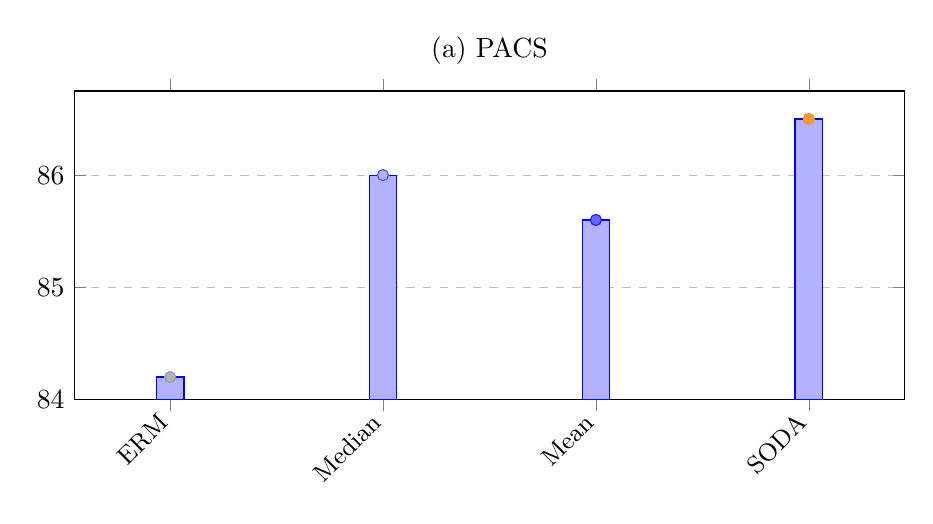
\begin{tikzpicture}
            \begin{axis}[stats multiplot style, title={(a) PACS}, ymin=84]
                \addplot+[scatter, scatter src=explicit symbolic] 
                table [meta=class, col sep=comma] {
                    x,      y,      class
                    ERM,    84.2,   ERM_class
                    Median, 86.0,   median_class
                    Mean,   85.6,   mean_class
                    SODA,   86.5,   soda_class
                };
            \end{axis}
        \end{tikzpicture}
    \end{subfigure}
    \hfill
    \begin{subfigure}{0.32\textwidth}
        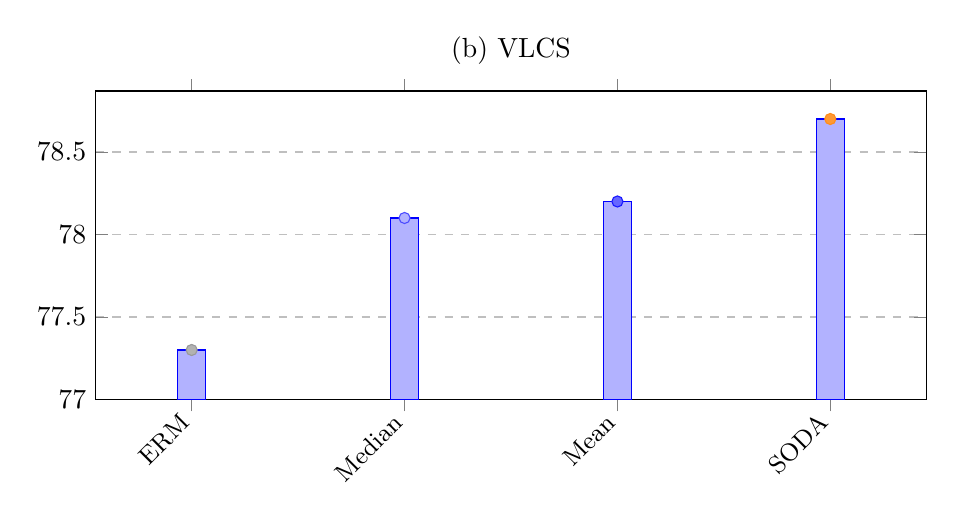
\begin{tikzpicture}
            \begin{axis}[stats multiplot style, title={(b) VLCS}, ymin=77]
                \addplot+[scatter, scatter src=explicit symbolic] 
                table [meta=class, col sep=comma] {
                    x,      y,      class
                    ERM,    77.3,   ERM_class
                    Median, 78.1,   median_class
                    Mean,   78.2,   mean_class
                    SODA,   78.7,   soda_class
                };
            \end{axis}
        \end{tikzpicture}
    \end{subfigure}
    \hfill
    \begin{subfigure}{0.32\textwidth}
        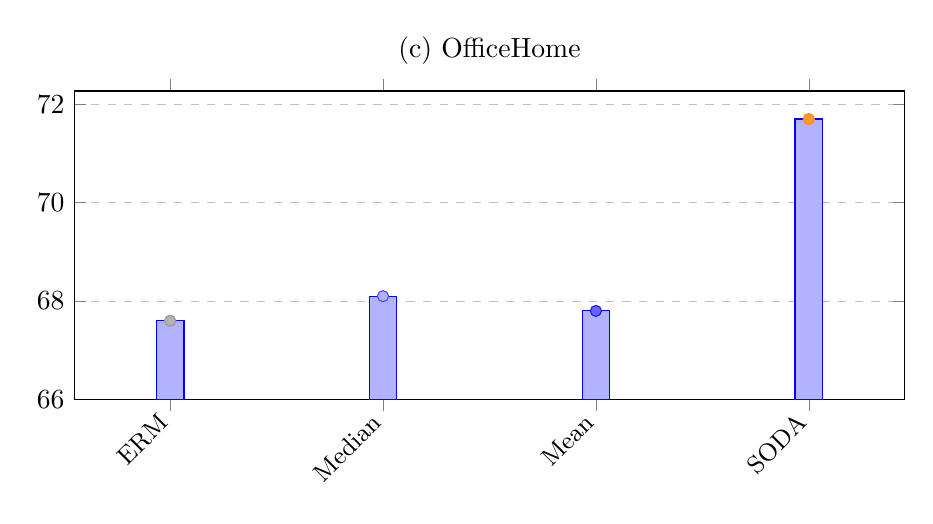
\begin{tikzpicture}
            \begin{axis}[stats multiplot style, title={(c) OfficeHome}, ymin=66]
                \addplot+[scatter, scatter src=explicit symbolic] 
                table [meta=class, col sep=comma] {
                    x,      y,      class
                    ERM,    67.6,   ERM_class
                    Median, 68.1,   median_class
                    Mean,   67.8,   mean_class
                    SODA,   71.7,   soda_class
                };
            \end{axis}
        \end{tikzpicture}
    \end{subfigure}

    \vspace{0.5cm}

    \begin{subfigure}{0.32\textwidth}
        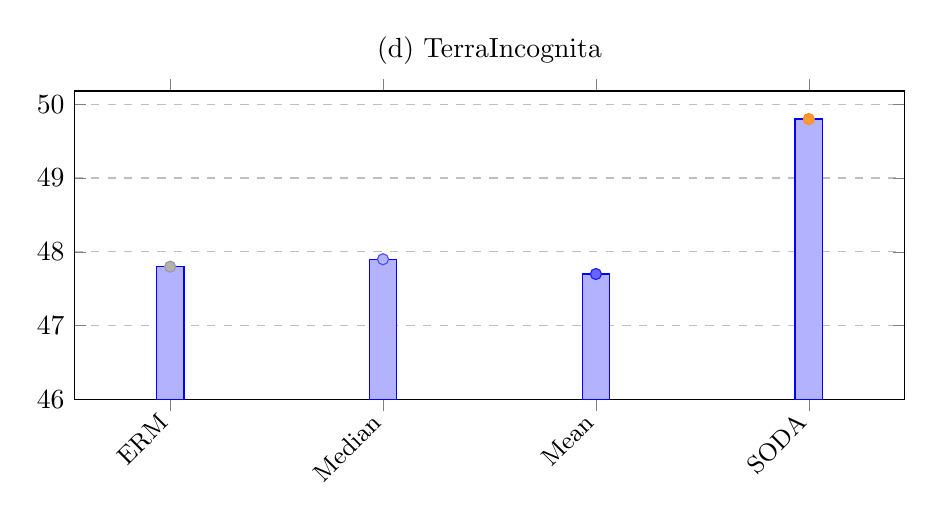
\begin{tikzpicture}
            \begin{axis}[stats multiplot style, title={(d) TerraIncognita}, ymin=46]
                \addplot+[scatter, scatter src=explicit symbolic] 
                table [meta=class, col sep=comma] {
                    x,      y,      class
                    ERM,    47.8,   ERM_class
                    Median, 47.9,   median_class
                    Mean,   47.7,   mean_class
                    SODA,   49.8,   soda_class
                };
            \end{axis}
        \end{tikzpicture}
    \end{subfigure}
    \hfill
    \begin{subfigure}{0.32\textwidth}
        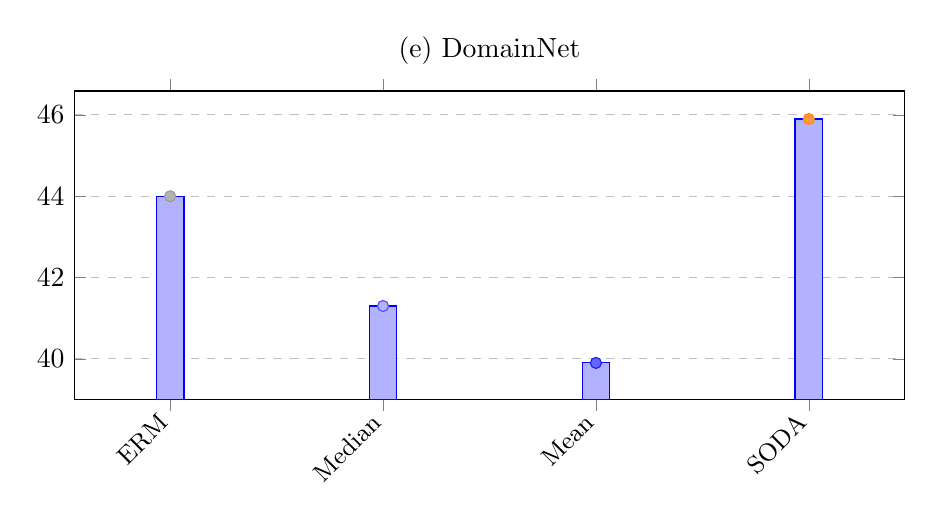
\begin{tikzpicture}
            \begin{axis}[stats multiplot style, title={(e) DomainNet}, ymin=39]
                \addplot+[scatter, scatter src=explicit symbolic] 
                table [meta=class, col sep=comma] {
                    x,      y,      class
                    ERM,    44.0,   ERM_class
                    Median, 41.3,   median_class
                    Mean,   39.9,   mean_class
                    SODA,   45.9,   soda_class
                };
            \end{axis}
        \end{tikzpicture}
    \end{subfigure}
    \hfill
    \begin{subfigure}{0.32\textwidth}
        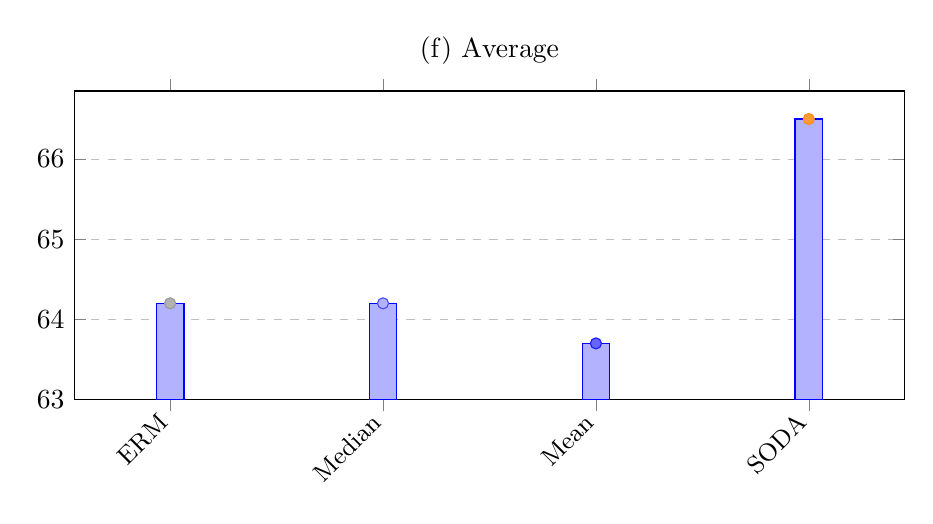
\begin{tikzpicture}
            \begin{axis}[stats multiplot style, title={(f) Average}, ymin=63]
                \addplot+[scatter, scatter src=explicit symbolic] 
                table [meta=class, col sep=comma] {
                    x,      y,      class
                    ERM,    64.2,   ERM_class
                    Median, 64.2,   median_class
                    Mean,   63.7,   mean_class
                    SODA,   66.5,   soda_class
                };
            \end{axis}
        \end{tikzpicture}
    \end{subfigure}

    \caption{Performance of SODA compared against the ERM baseline and the statistical distribution (Mean, Median) of eight state-of-the-art methods across all benchmarks. 
    The figure highlights SODA's robust performance; it consistently surpasses the average and median baseline accuracy. On key challenging datasets like OfficeHome and on the overall Average, it achieves a new state-of-the-art, demonstrating the effectiveness of the stabilized alignment strategy.}
    \label{fig:all_results_stats}
\end{figure*}